\documentclass[ngerman, a4paper, 12pt]{article}  
\usepackage{babel}

\usepackage{siunitx}  
\sisetup{locale = DE}

\usepackage{pgfplots}

\usepackage{geometry,lipsum}
\geometry{margin=1in}

\usepackage{enumitem}


\begin{document}

\begin{center}
    \huge \bf{Rutschenmodellierer}\\
    \footnotesize{Aufgabe erstellt von Jonas, Paul, Dominik}
\end{center}

\vspace{1.5cm}

Die beliebteste Attraktion der Stadt Bielefeld im Sommer,
wenn die Temperatur über 30°C liegt,
ist die Rutsche im Südschwimmbad.
Der Bademeister Jochen Jürgen hat sich aus Langeweile
aufgrund der wenigen Kundschaft in den Morgenstunden eine Funktion $r$ überlegt,
die im zweiten Quadranten eines kartesischen Koordinatensystems den Längenquerschnitt der Rutsche modelliert.
Die Modellierung besteht hier aus der hochmodernen, harmonisch geformten Treppe links
und der eigentlichen Rutschbahn rechts.
Von der Baufirma des Auffangbeckens \textit{Schwimmbecken Liebreich GmbH}
hat er außerdem die Modellierung dieses Beckens mit der Funktion $b$ erhalten:

$$r(x) = -0,1x^4 - 0,5x^3 - 0,1x^2$$
$$b(x) = 0,2x^2 - 5$$

In fleißiger Arbeit hat sich der 20-jährige Schwimmwart die Funktion $b$ dabei so modelliert,
dass sie den Boden hinter der Rutsche im vierten Quadranten (ebenfalls im Querschnitt) anzeigt.
Die beiden Funktionen stellen nun jede Koordinaten-Einheit als einen realen Meter dar.
Bevor er es versehentlich auf den Boden fallengelassen und es völlig durchnässt wurde,
hatte Herr Jürgen außerdem einen selbstgezeichneten Plot seiner beiden Funktionen auf einem Papier:

\begin{figure}[h]
    \centering
    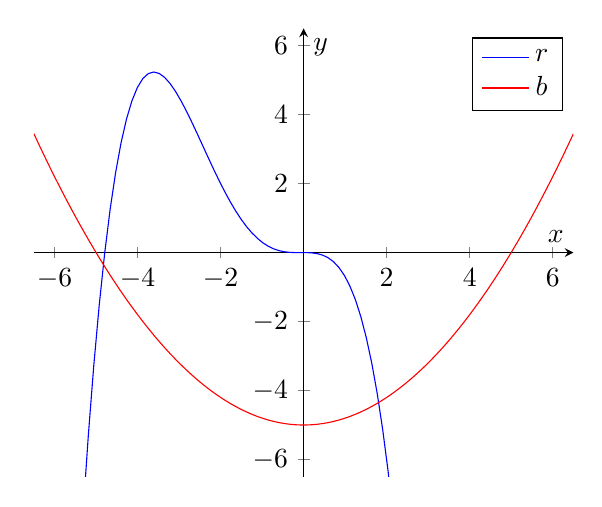
\begin{tikzpicture}
        \begin{axis}[
            axis lines = middle,
            xlabel = $x$,
            ylabel = $y$,
            xmin=-6.5, xmax=6.5,
            ymin=-6.5, ymax=6.5,
        ]
            \addplot [domain=-6.5:6.5, samples=100, color=blue]{-0.1*x^4 -0.5*x^3 -0.1*x^2};
            \addlegendentry{\(r\)}
            \addplot [domain=-6.5:6.5, samples=100, color=red]{0.2*x^2 -5};
            \addlegendentry{\(b\)}
        \end{axis}
    \end{tikzpicture}
\end{figure}

Als der Schwimmmeister ein paar Jugendliche über ihre Lehrkräfte diskutieren hört,
erinnert er sich an seine Schulzeit und die anwendungsbezogenen Aufgaben des Mathematik-Unterrichts.
Schnell erstellt der Experte eine Liste an Aufgaben. Lösen Sie die folgenden Aufgaben!

\begin{enumerate}
    \item[a)]
        \begin{enumerate}
            \item[(i)]
                Bestimmen Sie rechnerisch die Länge und die maximale Tiefe (direkt nach Ende der Rutsche) des Auffangbeckens.
            \item[(ii)]
                Berechnen Sie den Wasseroberflächeninhalt unter der Ahnnahme,
                dass das Becken im dreidimensionalen Raum mit einer hinzugedachten $z$-Achse,
                die senkrecht zu den $x$- und $y$-Achsen steht, rotationssymmetrisch zur $y$-Achse ist.
                Die Oberfläche des Beckens ist in diesem Gedankenbild also halbkreisförmig und liegt an der $z$-Achse.
                Schätzen Sie außerdem begründet die nächste ganze Zahl ab, die dem berechneten Wert am nächsten liegt.\\
                (Zur Kontrolle: Der Oberflächeninhalt des Beckens beträgt circa $\SI{39}{\square\metre}$.)
        \end{enumerate}
        \begin{flushright}
            (x+x Punkte)
        \end{flushright}
    \item[b)]
        \begin{enumerate}
            \item[(i)]
                Ermitteln Sie rechnerisch die Nullstellen
                sowie die Koordinaten und die Art der Extrem- und Wendepunkte von $r$ und $b$
                und zeigen Sie, dass es sich bei der Wendestelle um eine Sattelstelle handelt.
            \item[(ii)]
                Erklären Sie die Bedeutung aller dieser Stellen im Sachzusammenhang.
        \end{enumerate}
\end{enumerate}

Da Jürgens Vorgesetzter bei seinem letzten Rundgang auf den großzügigen Raum unter der Rutsche aufmerksam geworden ist,
schlägt er vor, dort Brennholz für die altmodische Wasser-Beheizungsanlage zu verstauen.
Dem Bademeister wurde so die Aufgabe deligiert, eine Schätzung für den vorhandenen Raum unter der Rutsche abzugeben.
Die besondere Rutsche hat am Fuß der Leiter eine Breite von lediglich einem Meter und wird linear breiter
bis sie am Ende, also an der Kante am Beckenrand, eine Breite von stolzen drei Metern erreicht,
was es zum Misfallen des Schwimmwarts ermöglicht, mit mehreren Leuten gleichzeitig zu rutschen.

\begin{enumerate}[resume]
    \item[]
        \begin{enumerate}[resume]
            \item[(iii)]
                Bestimmen Sie das Volumen des möglichen Stauraums unter der Annahme,
                dass der Graph von $r$ auch gleichzeitig ideal die Decke dieses Raums darstellt,
                und erläutern Sie Ihr Vorgehen.
        \end{enumerate}
        \begin{flushright}
            (x+x+x Punkte)
        \end{flushright}
\end{enumerate}

Die Form der Rutsche, die der renommierte Designer S. Altrock übernommen hat, hat leider ein Defizit:
Jochen Jürgen muss nämlich in seinem Beruf leider täglich Kinder beobachten, die auf der Leiter ausrutschen.
Da er dies durch seine scharfe Beobachtungsgabe auf die besondere Form zurückzuführen meint, plant er eine neue, gerade Leiter.
Die Neigung soll exakt 80° betragen.

\begin{enumerate}[resume]
    \item[c)]
        \begin{enumerate}
            \item[(i)]
                Ermitteln Sie eine Funktionsgleichung der Geraden $l$,
                die in Relation zu den bereits gegebenen Graphen die neue Leiter modelliert.
            \item[(ii)]
                Bestimmen Sie die Länge der Leiter.
        \end{enumerate}
        \begin{flushright}
            (x+x Punkte)
        \end{flushright}
\end{enumerate}

\end{document}
